\documentclass[tikz,border=2pt]{standalone}
\usepackage{tikz}
\usetikzlibrary{positioning}
\begin{document}
% Namikawa--Ueno type: 2II^*-t
% Target MRNC type: 2II^*-t
% Adapted from Tim Dokchitser picture: [2]II^*_{{\it n}D}
% Parameter substitution: n -> t
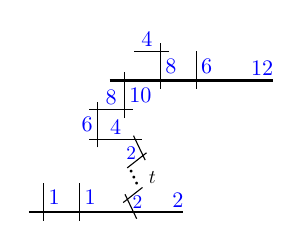
\begin{tikzpicture}[xscale=0.57,yscale=0.62]
\draw[thick,shorten >=2] (-1/3,0)--(97/30,0) node[inner sep=2pt,blue,above left,scale=0.8] {2};
\draw[shorten <=-3pt] (0,0)--node[inner sep=2pt,scale=0.8,blue,right] {1} (0,3/5);
\draw[shorten <=-3pt] (4/5,0)--node[inner sep=2pt,scale=0.8,blue,right] {1} (4/5,3/5);
\draw (2,0) 
    ++(0.07,-0.13)--++(-0.26,0.5)++(0.12,-0.19)  
    ++(0,0.02)
      node[blue,scale=0.7,inner sep=1,anchor=west]{2}
    ++(0,-0.02)
    ++(-0.16,0.02)--++(0.43,0.31)++(-0.13,0.07)  
    node{$\cdot$} ++(-0.06,0.12) node{$\cdot$}
    ++(-0.06,0.12) node{$\cdot$}++(0.17,-0.1)    node[auto,inner sep=5,scale=0.7,anchor=west]{$t$}
    ++(-0.26,0.19)--++(0.43,0.31)++(-0.18,0.04)   
    ++(0,-0.04)
      node[blue,scale=0.7,inner sep=1,anchor=east]{2}
    ++(0,0.04)
    ++(0.18,-0.04)++(-0.03,-0.15)--++(-0.26,0.5);
\draw[shorten <=-3pt, shorten >=-3pt] (2,3/2)--node[inner sep=2pt,scale=0.8,blue,above] {4} (6/5,3/2);
\draw[shorten <=-3pt, shorten >=-3pt] (6/5,3/2)--node[inner sep=2pt,scale=0.8,blue,left] {6} (6/5,21/10);
\draw[shorten <=-3pt, shorten >=-3pt] (6/5,21/10)--node[inner sep=2pt,scale=0.8,blue,above] {8} (9/5,21/10);
\draw[shorten <=-3pt, shorten >=-3pt] (9/5,21/10)--node[inner sep=2pt,scale=0.8,blue,right] {10} (9/5,27/10);
\draw[thick,shorten >=2] (22/15,27/10)--(157/30,27/10) node[inner sep=2pt,blue,above left,scale=0.8] {12};
\draw[shorten <=-3pt, shorten >=-3pt] (13/5,27/10)--node[inner sep=2pt,scale=0.8,blue,right] {8} (13/5,33/10);
\draw[shorten <=-3pt] (13/5,33/10)--node[inner sep=2pt,scale=0.8,blue,above] {4} (2,33/10);
\draw[shorten <=-3pt] (17/5,27/10)--node[inner sep=2pt,scale=0.8,blue,right] {6} (17/5,33/10);
\end{tikzpicture}
\end{document}
